\section{Introduction to nonlinear Schwarz methods}
% TODO: maybe remove this slide.
\begin{frame}{Nonlinear domain decomposition methods}
	\begin{tikzpicture}[node distance=7cm]

		\node[inner sep=0pt] (one) at (-5,1.5){\Large\emph{\underline{Classical approach}}};
		\node[inner sep=0pt] (one) at (-5,0)
		{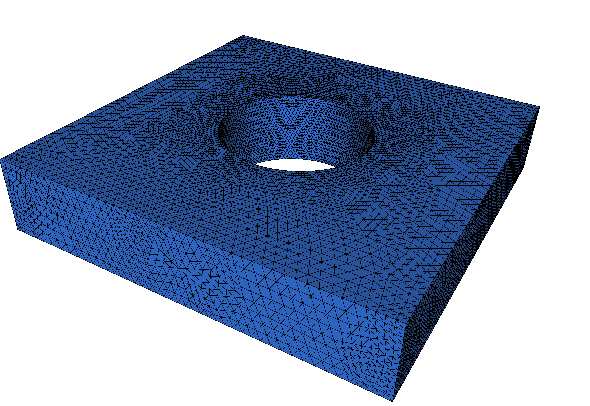
\includegraphics[width=2.9cm]{images/eps/rechteckring58534p_64001.pdf}};

		\node[inner sep=0pt] (two) at (-1,0)
		{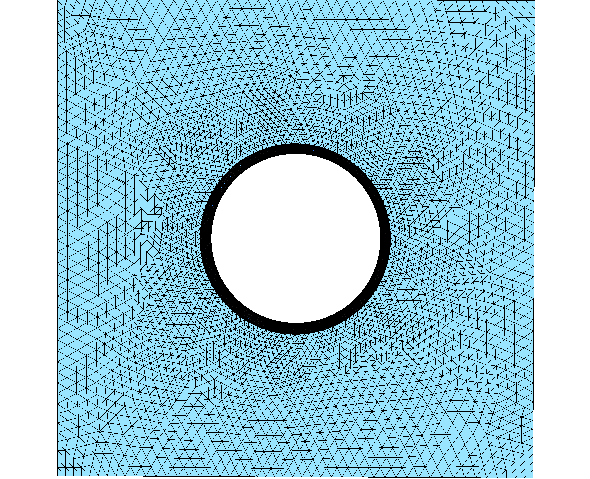
\includegraphics[width=2.2cm]{images/eps/rechteckring58534p_copy008.pdf}};
		\node[inner sep=0pt] (three) at (2.7,0)
		{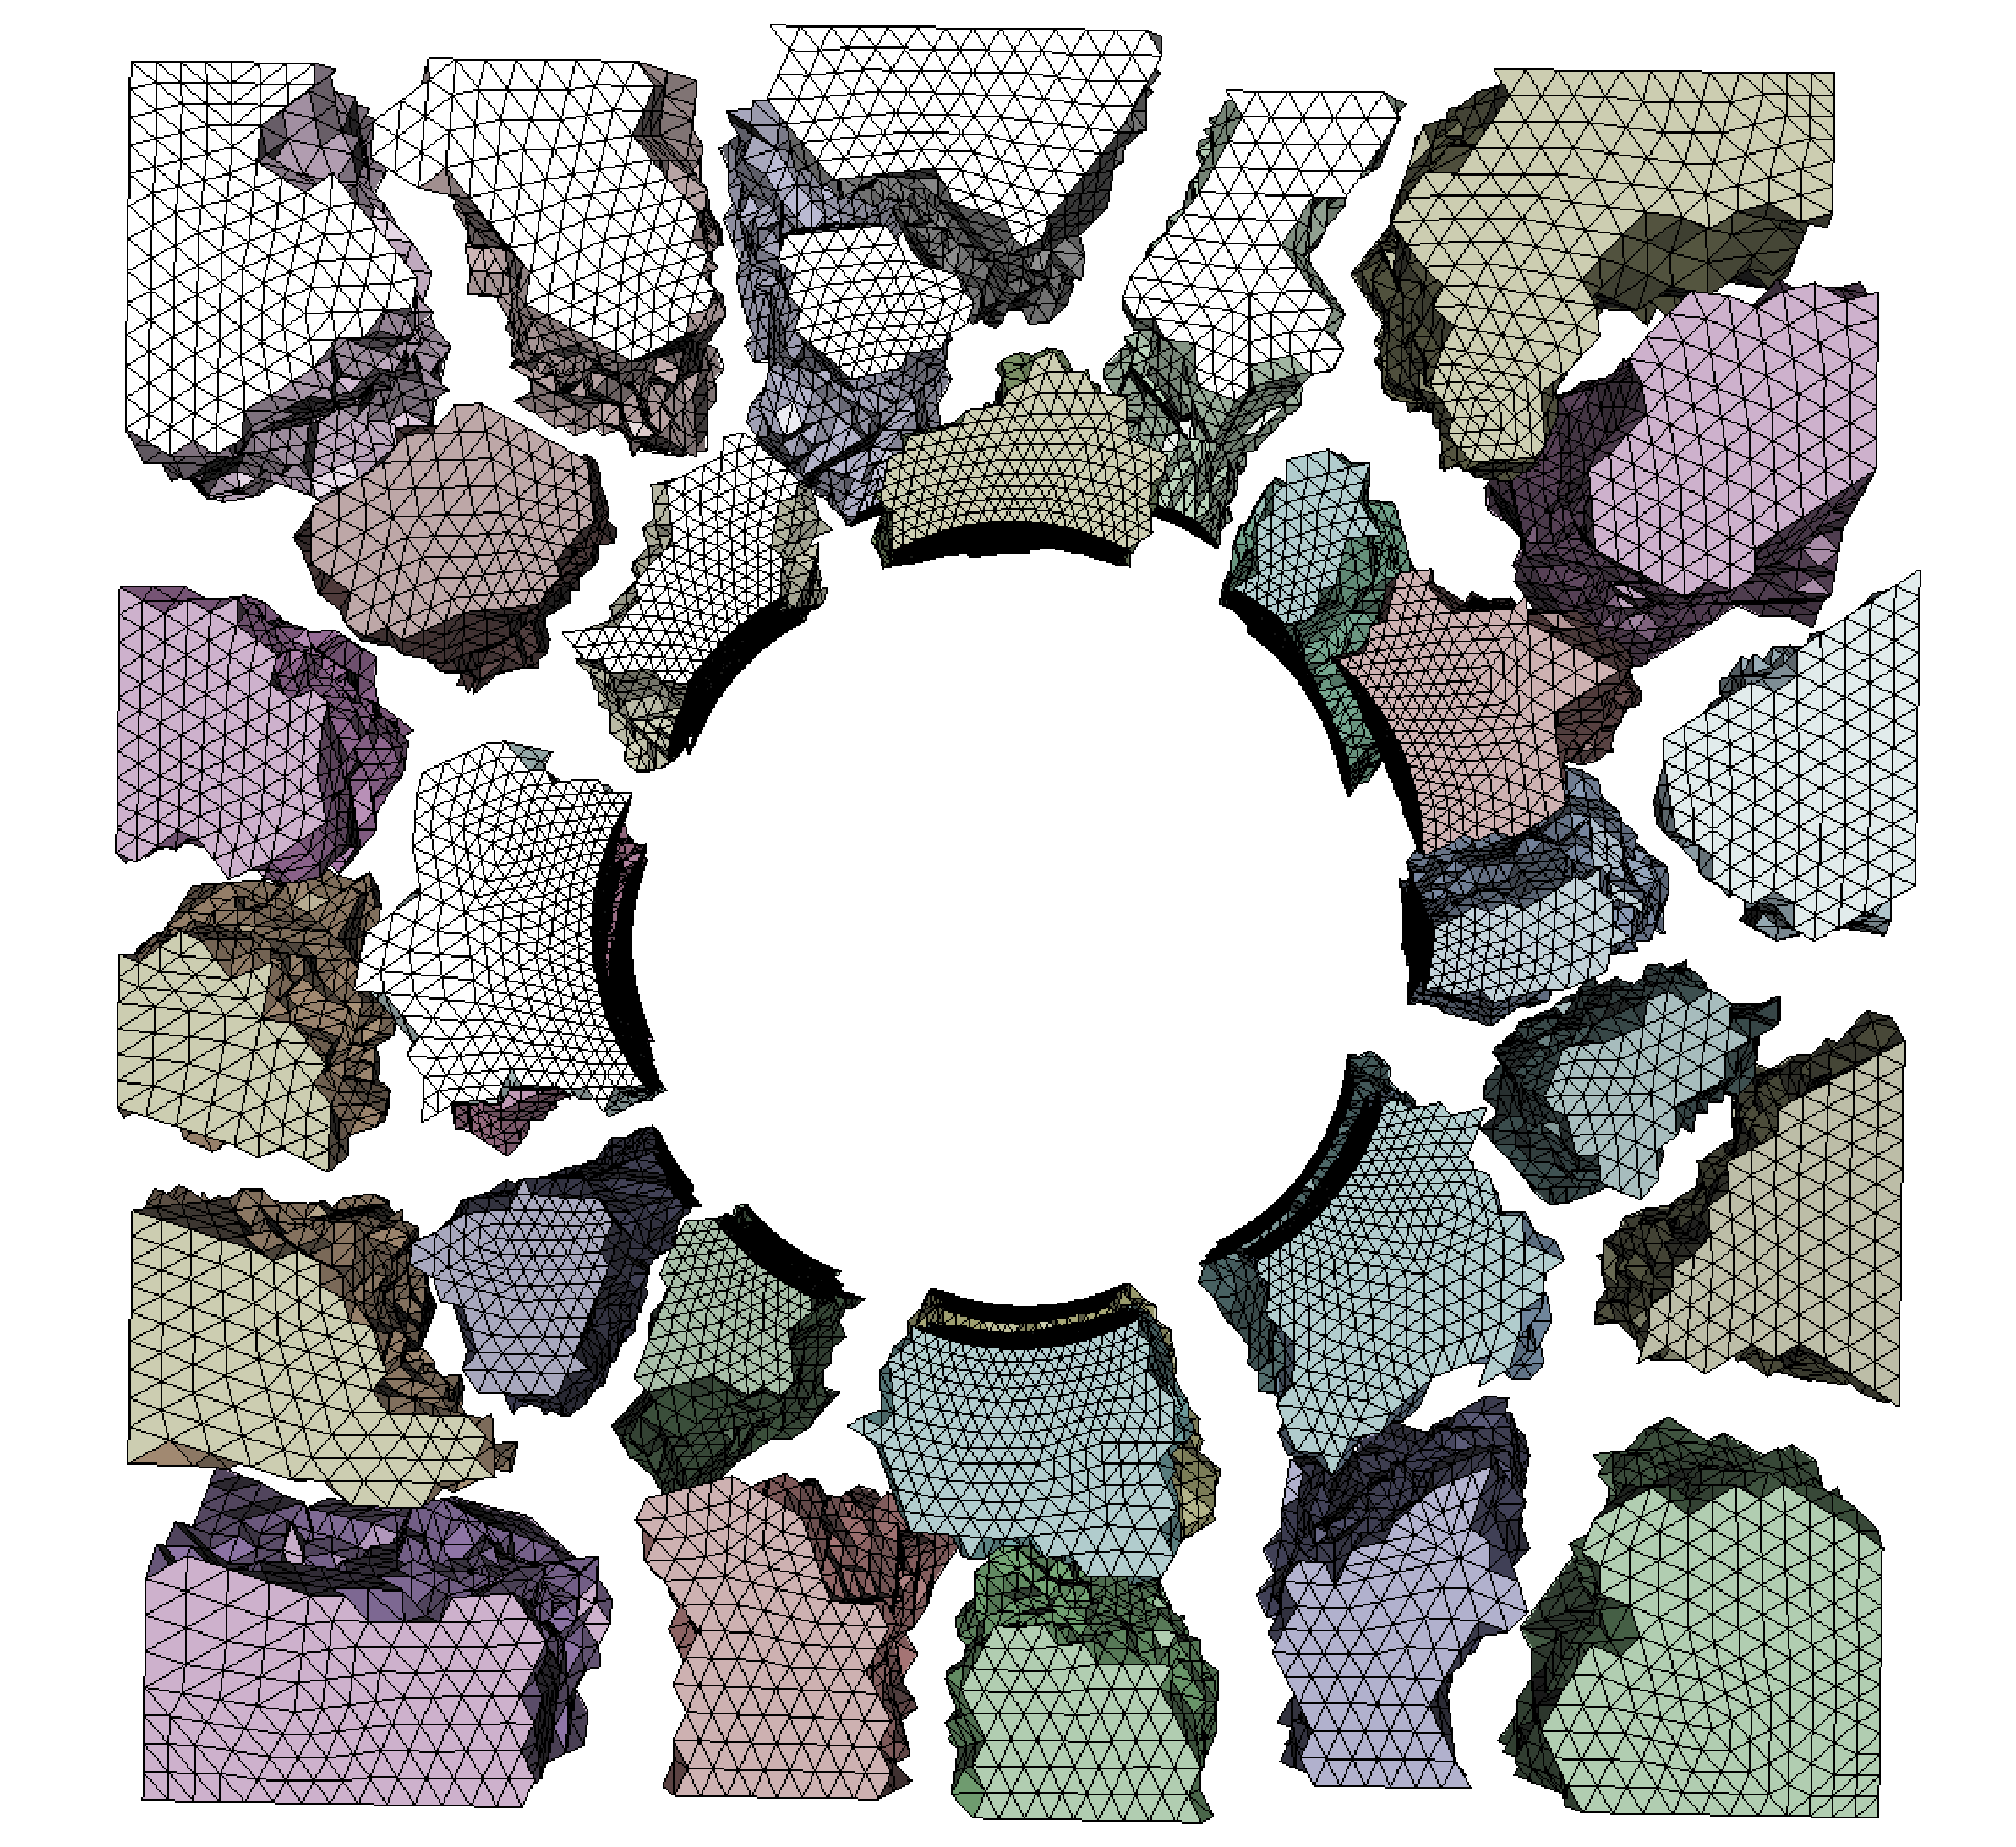
\includegraphics[width=2.0cm]{images/eps/exploded_5004_entsaettigt3.pdf}};
		\node[inner sep=0pt] (four) at (6,0)
		{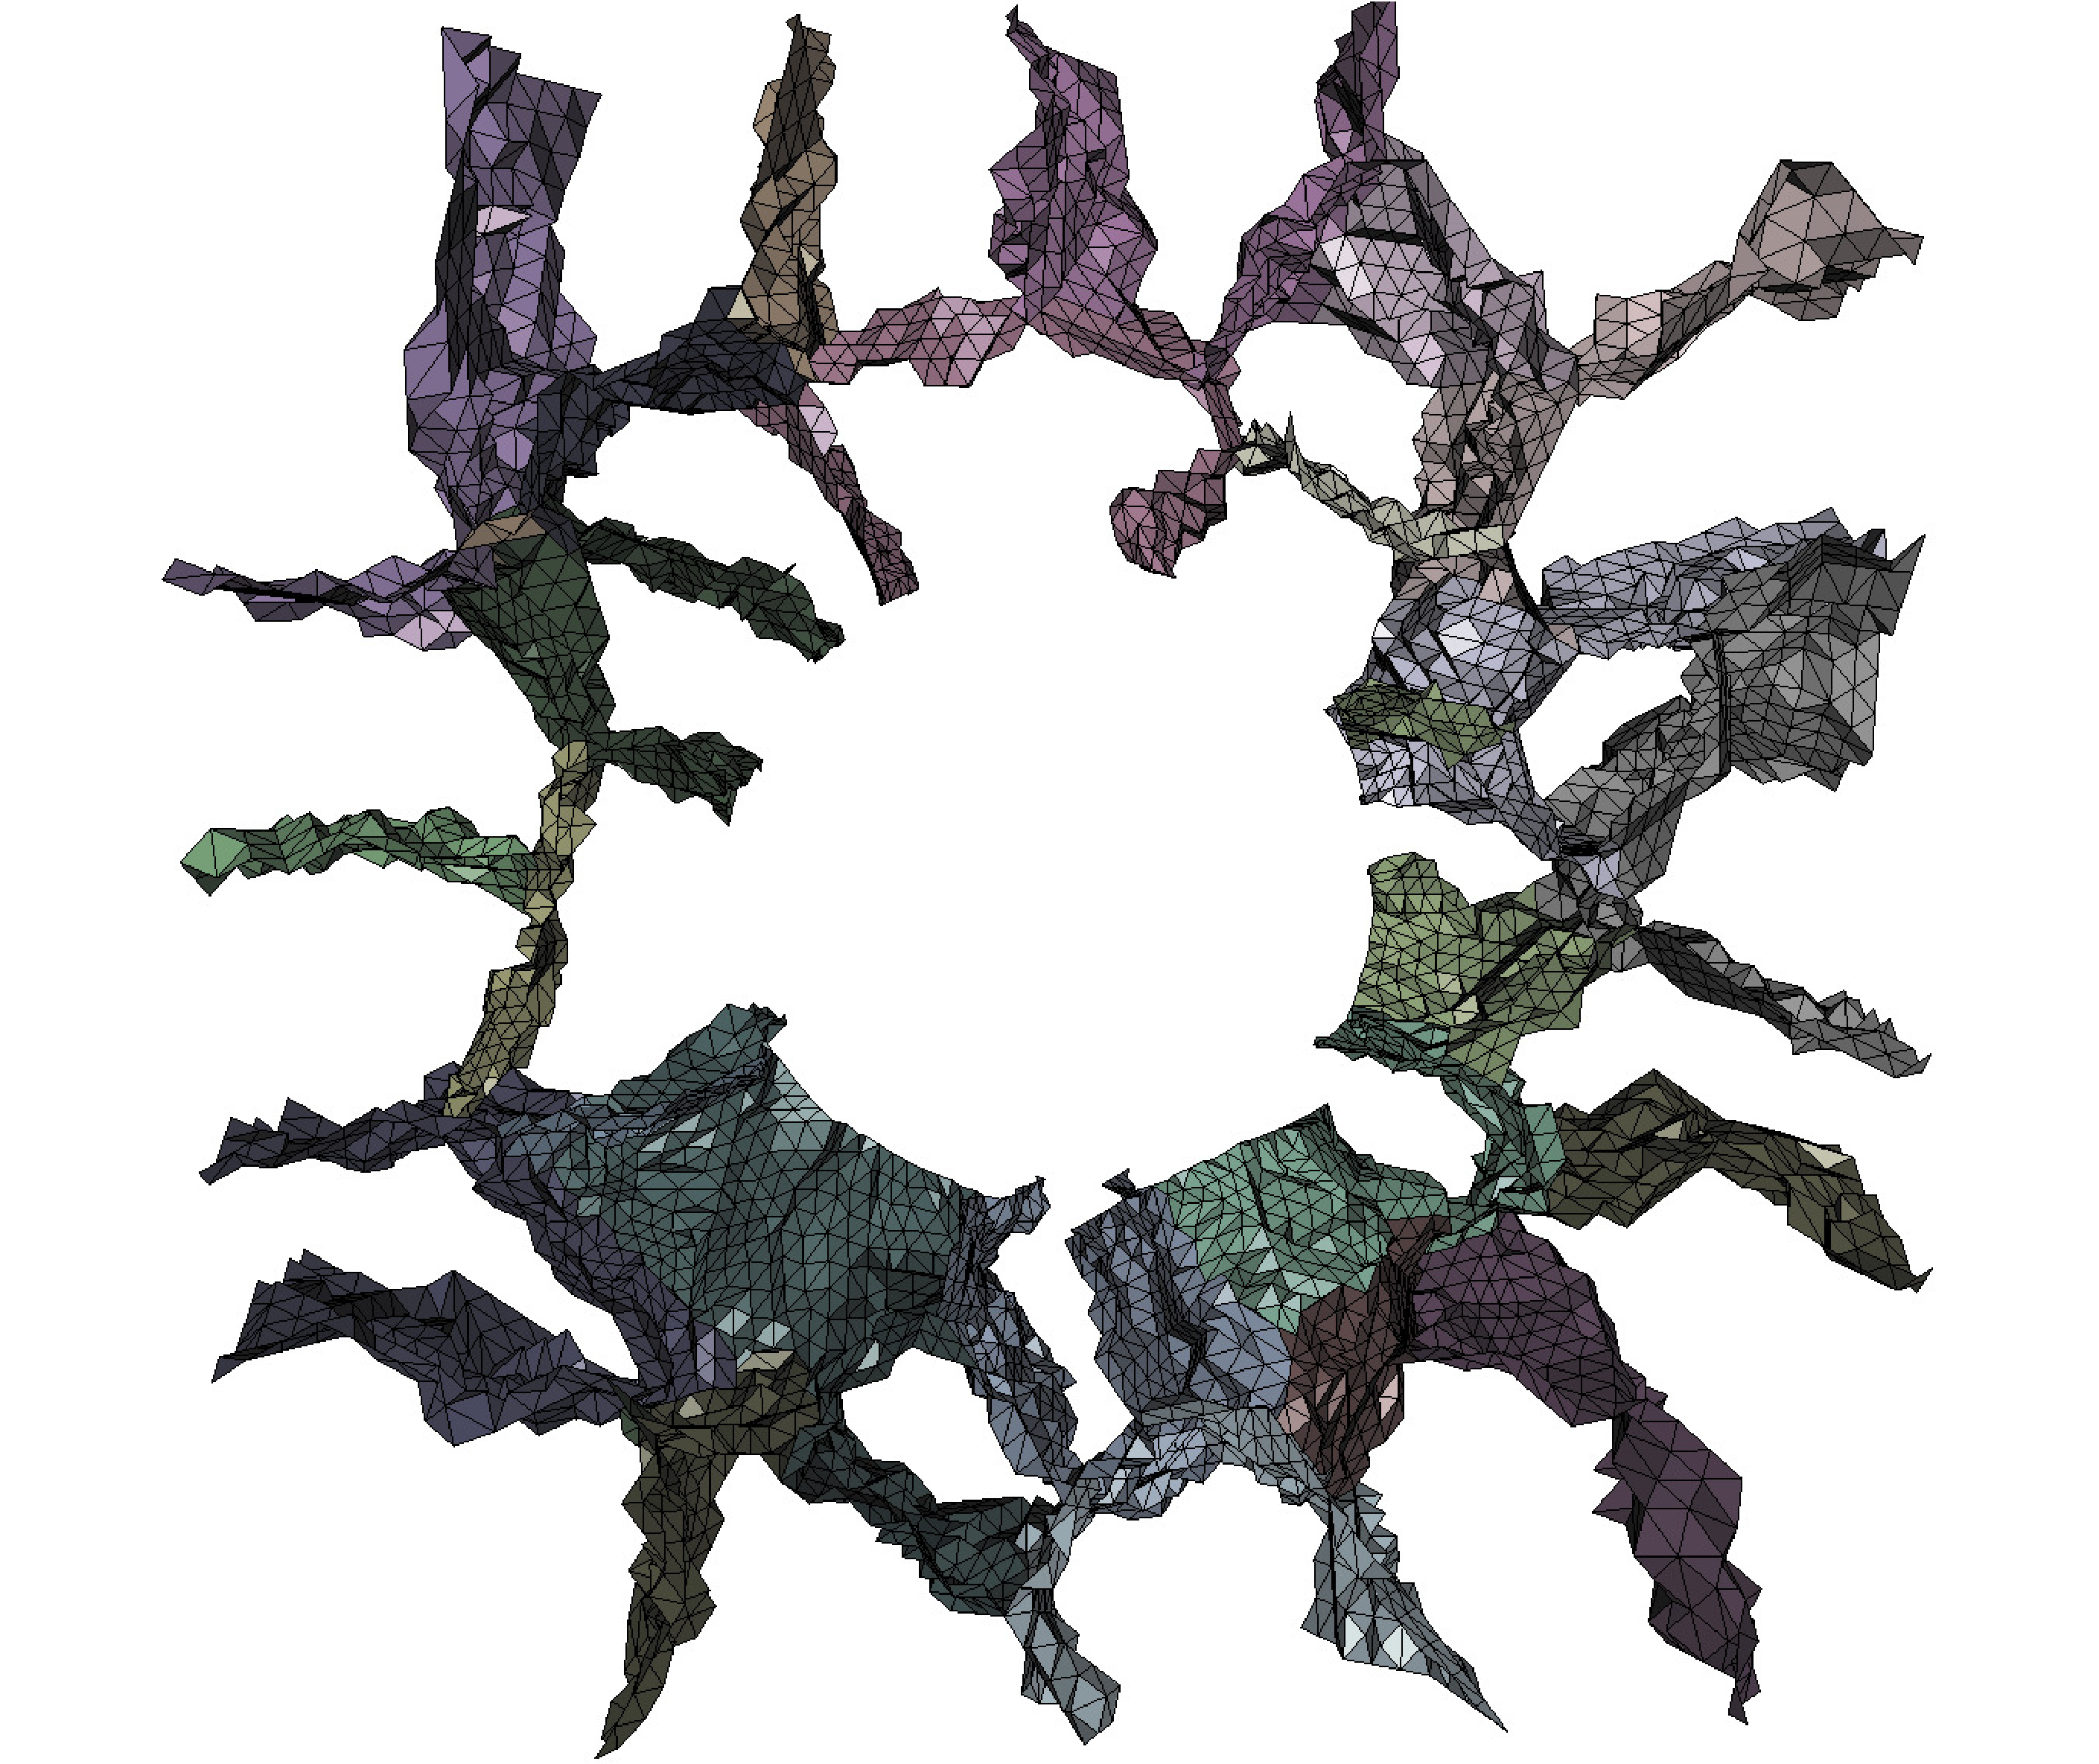
\includegraphics[width=2.3cm]{images/eps/rechteckring58534p_copy_entsaettigt3003.pdf}};

		\draw [arrow] (one) -- node[anchor=south] {\bf Linearize} (two);
		\draw [arrow] (two) -- node[anchor=south] {\bf Decompose} (three);
		\draw [arrow] (three) -- node[anchor=south] {\bf Build prec.} (four);
	\end{tikzpicture}

	\vspace*{1cm}
	\begin{tikzpicture}[node distance=2cm]

		\node[inner sep=0pt] (one) at (-4.4,1.5){\Large\emph{\underline{Nonlinear DD approach}}};
		\node[inner sep=0pt] (one) at (-5,0)
		{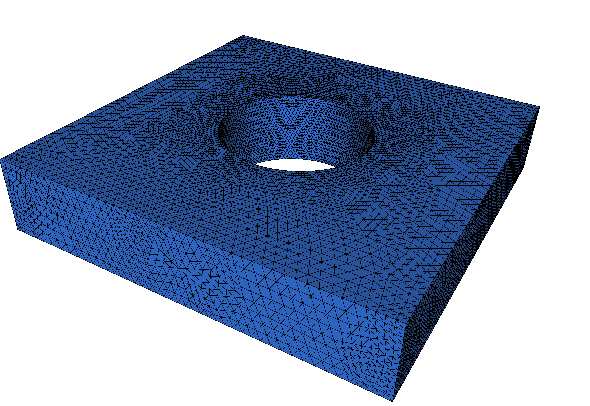
\includegraphics[width=2.9cm]{images/eps/rechteckring58534p_64001.pdf}};

		\node[inner sep=0pt] (two) at (-1,0)
		{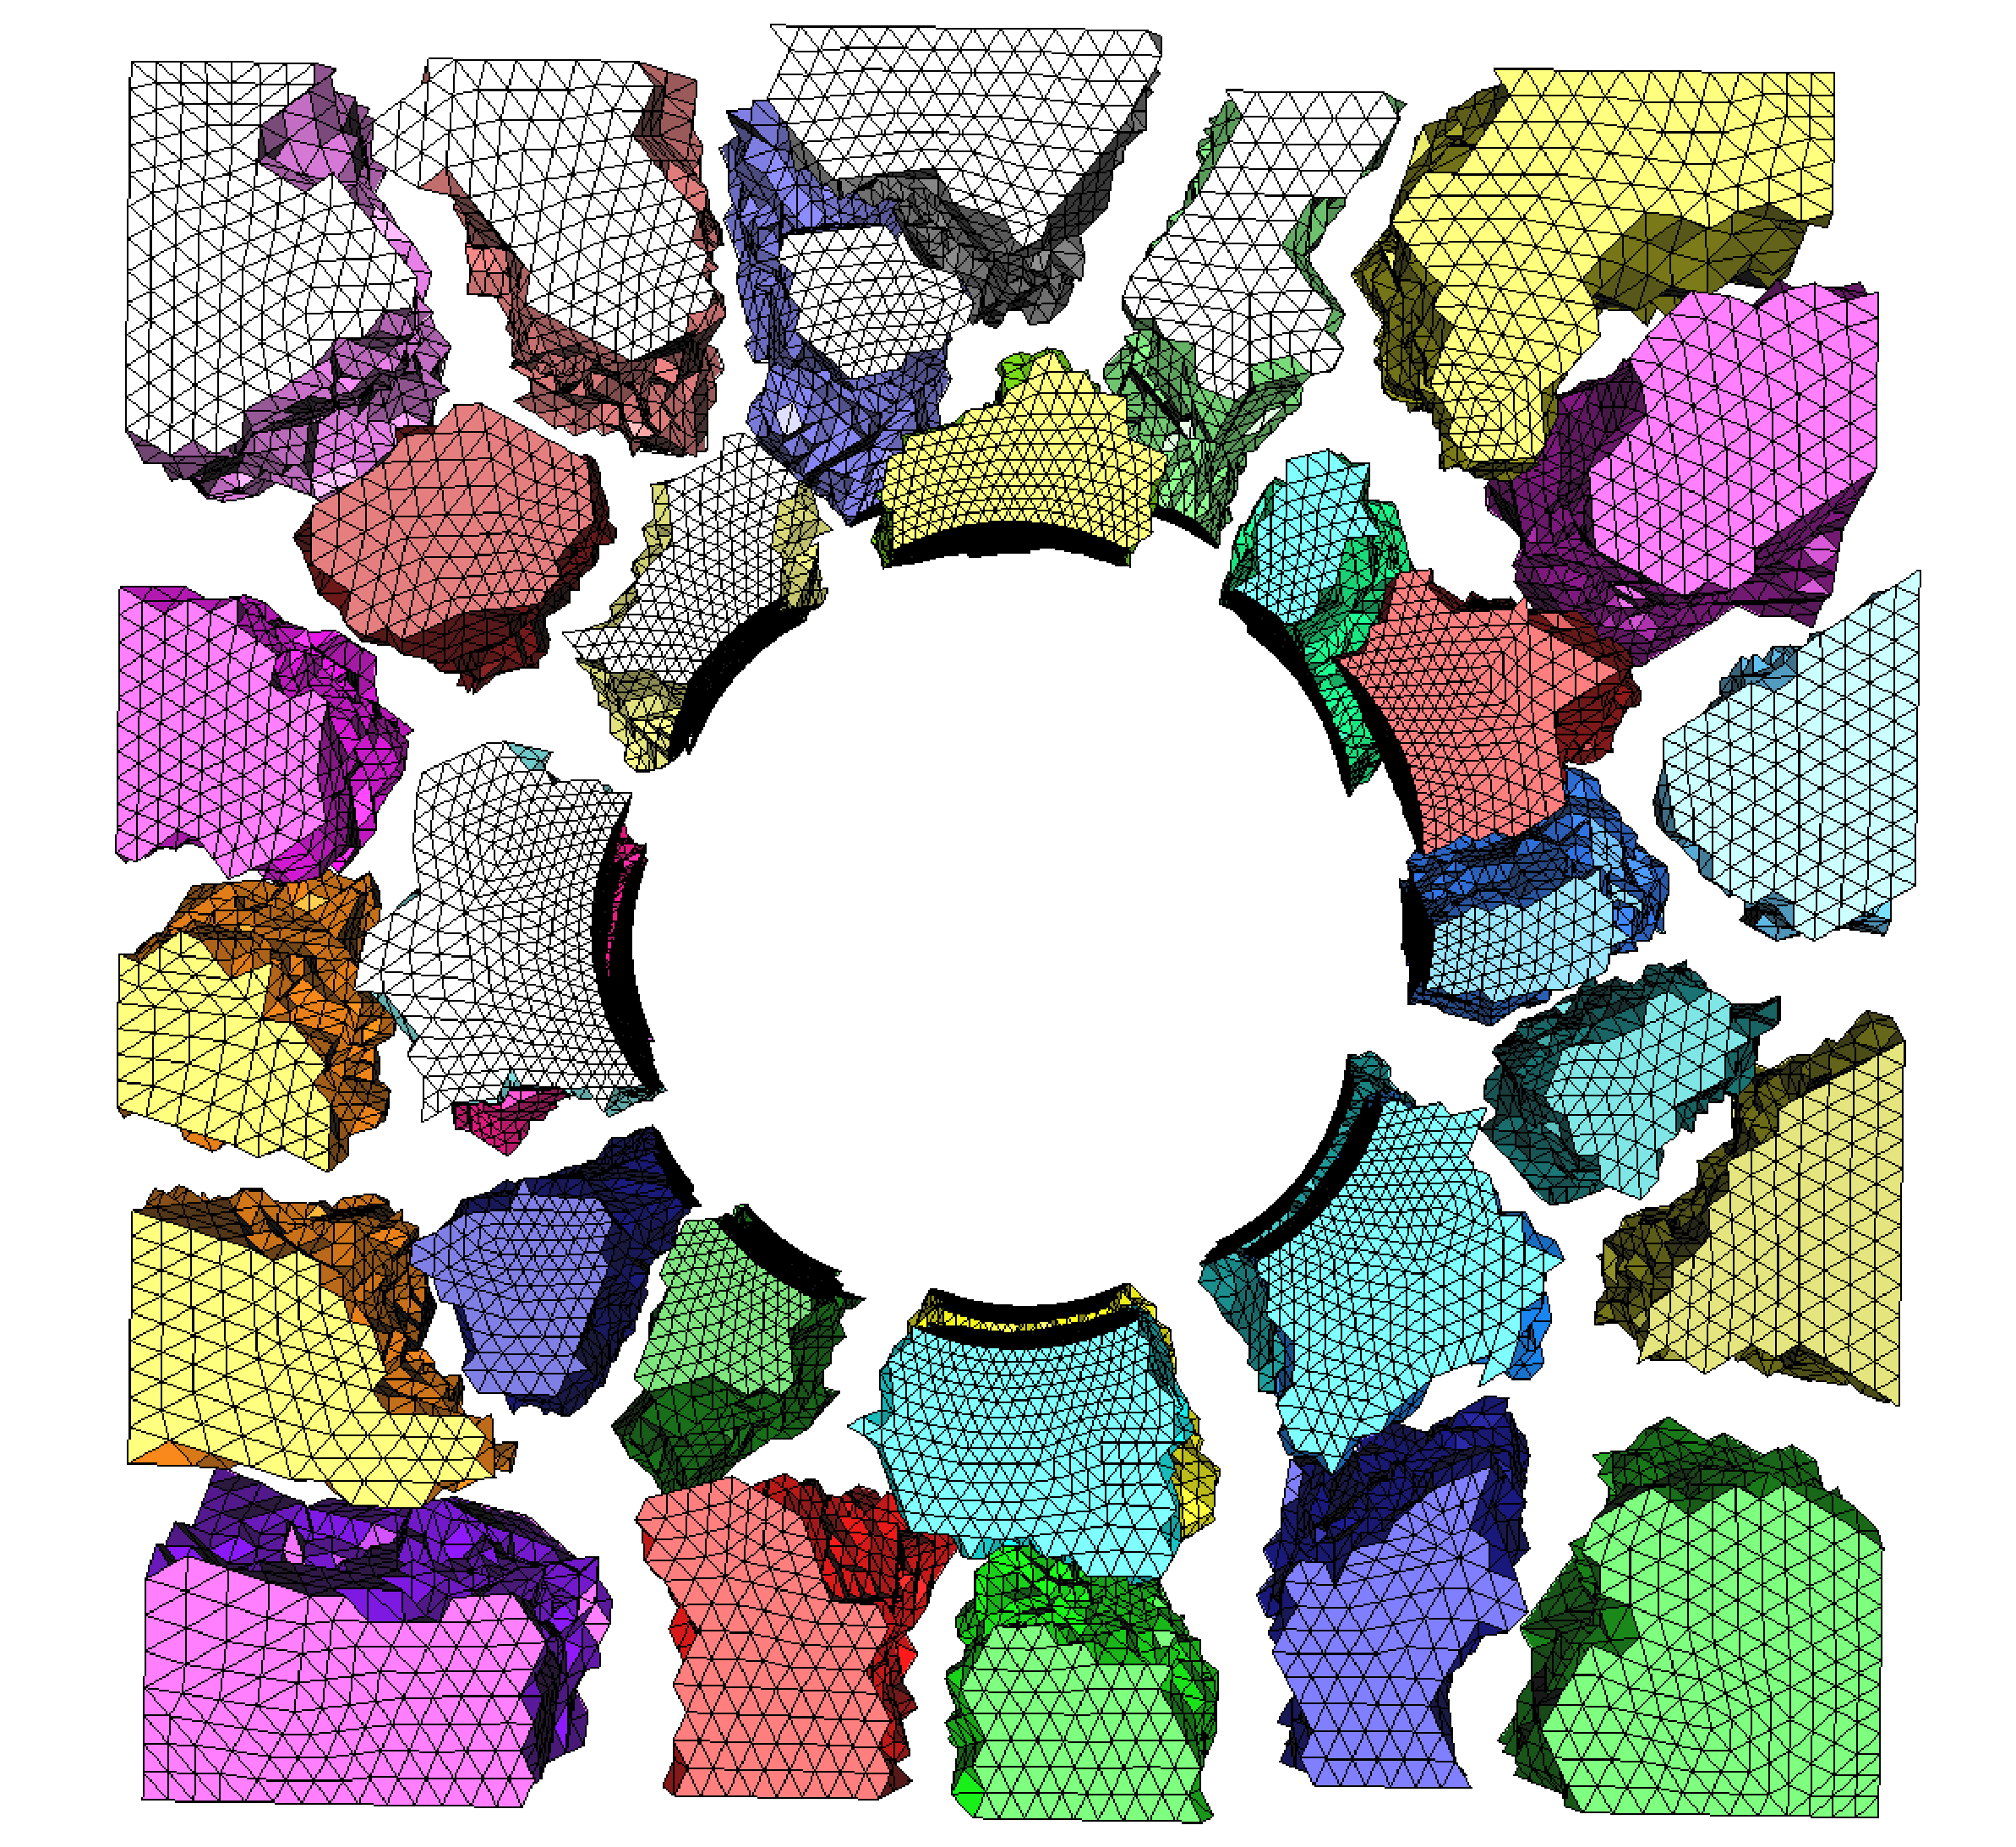
\includegraphics[width=2.0cm]{images/eps/exploded_5004.pdf}};
		\node[inner sep=0pt] (three) at (2.7,0)
		{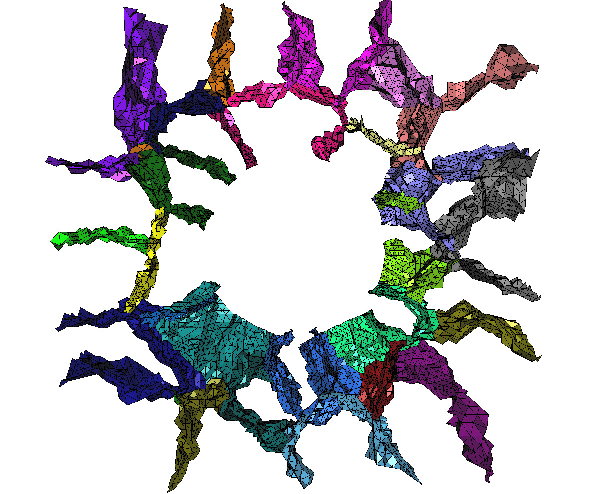
\includegraphics[width=2.3cm]{images/eps/rechteckring58534p_copy003.pdf}};
		\node[inner sep=0pt] (four) at (6,0)
		{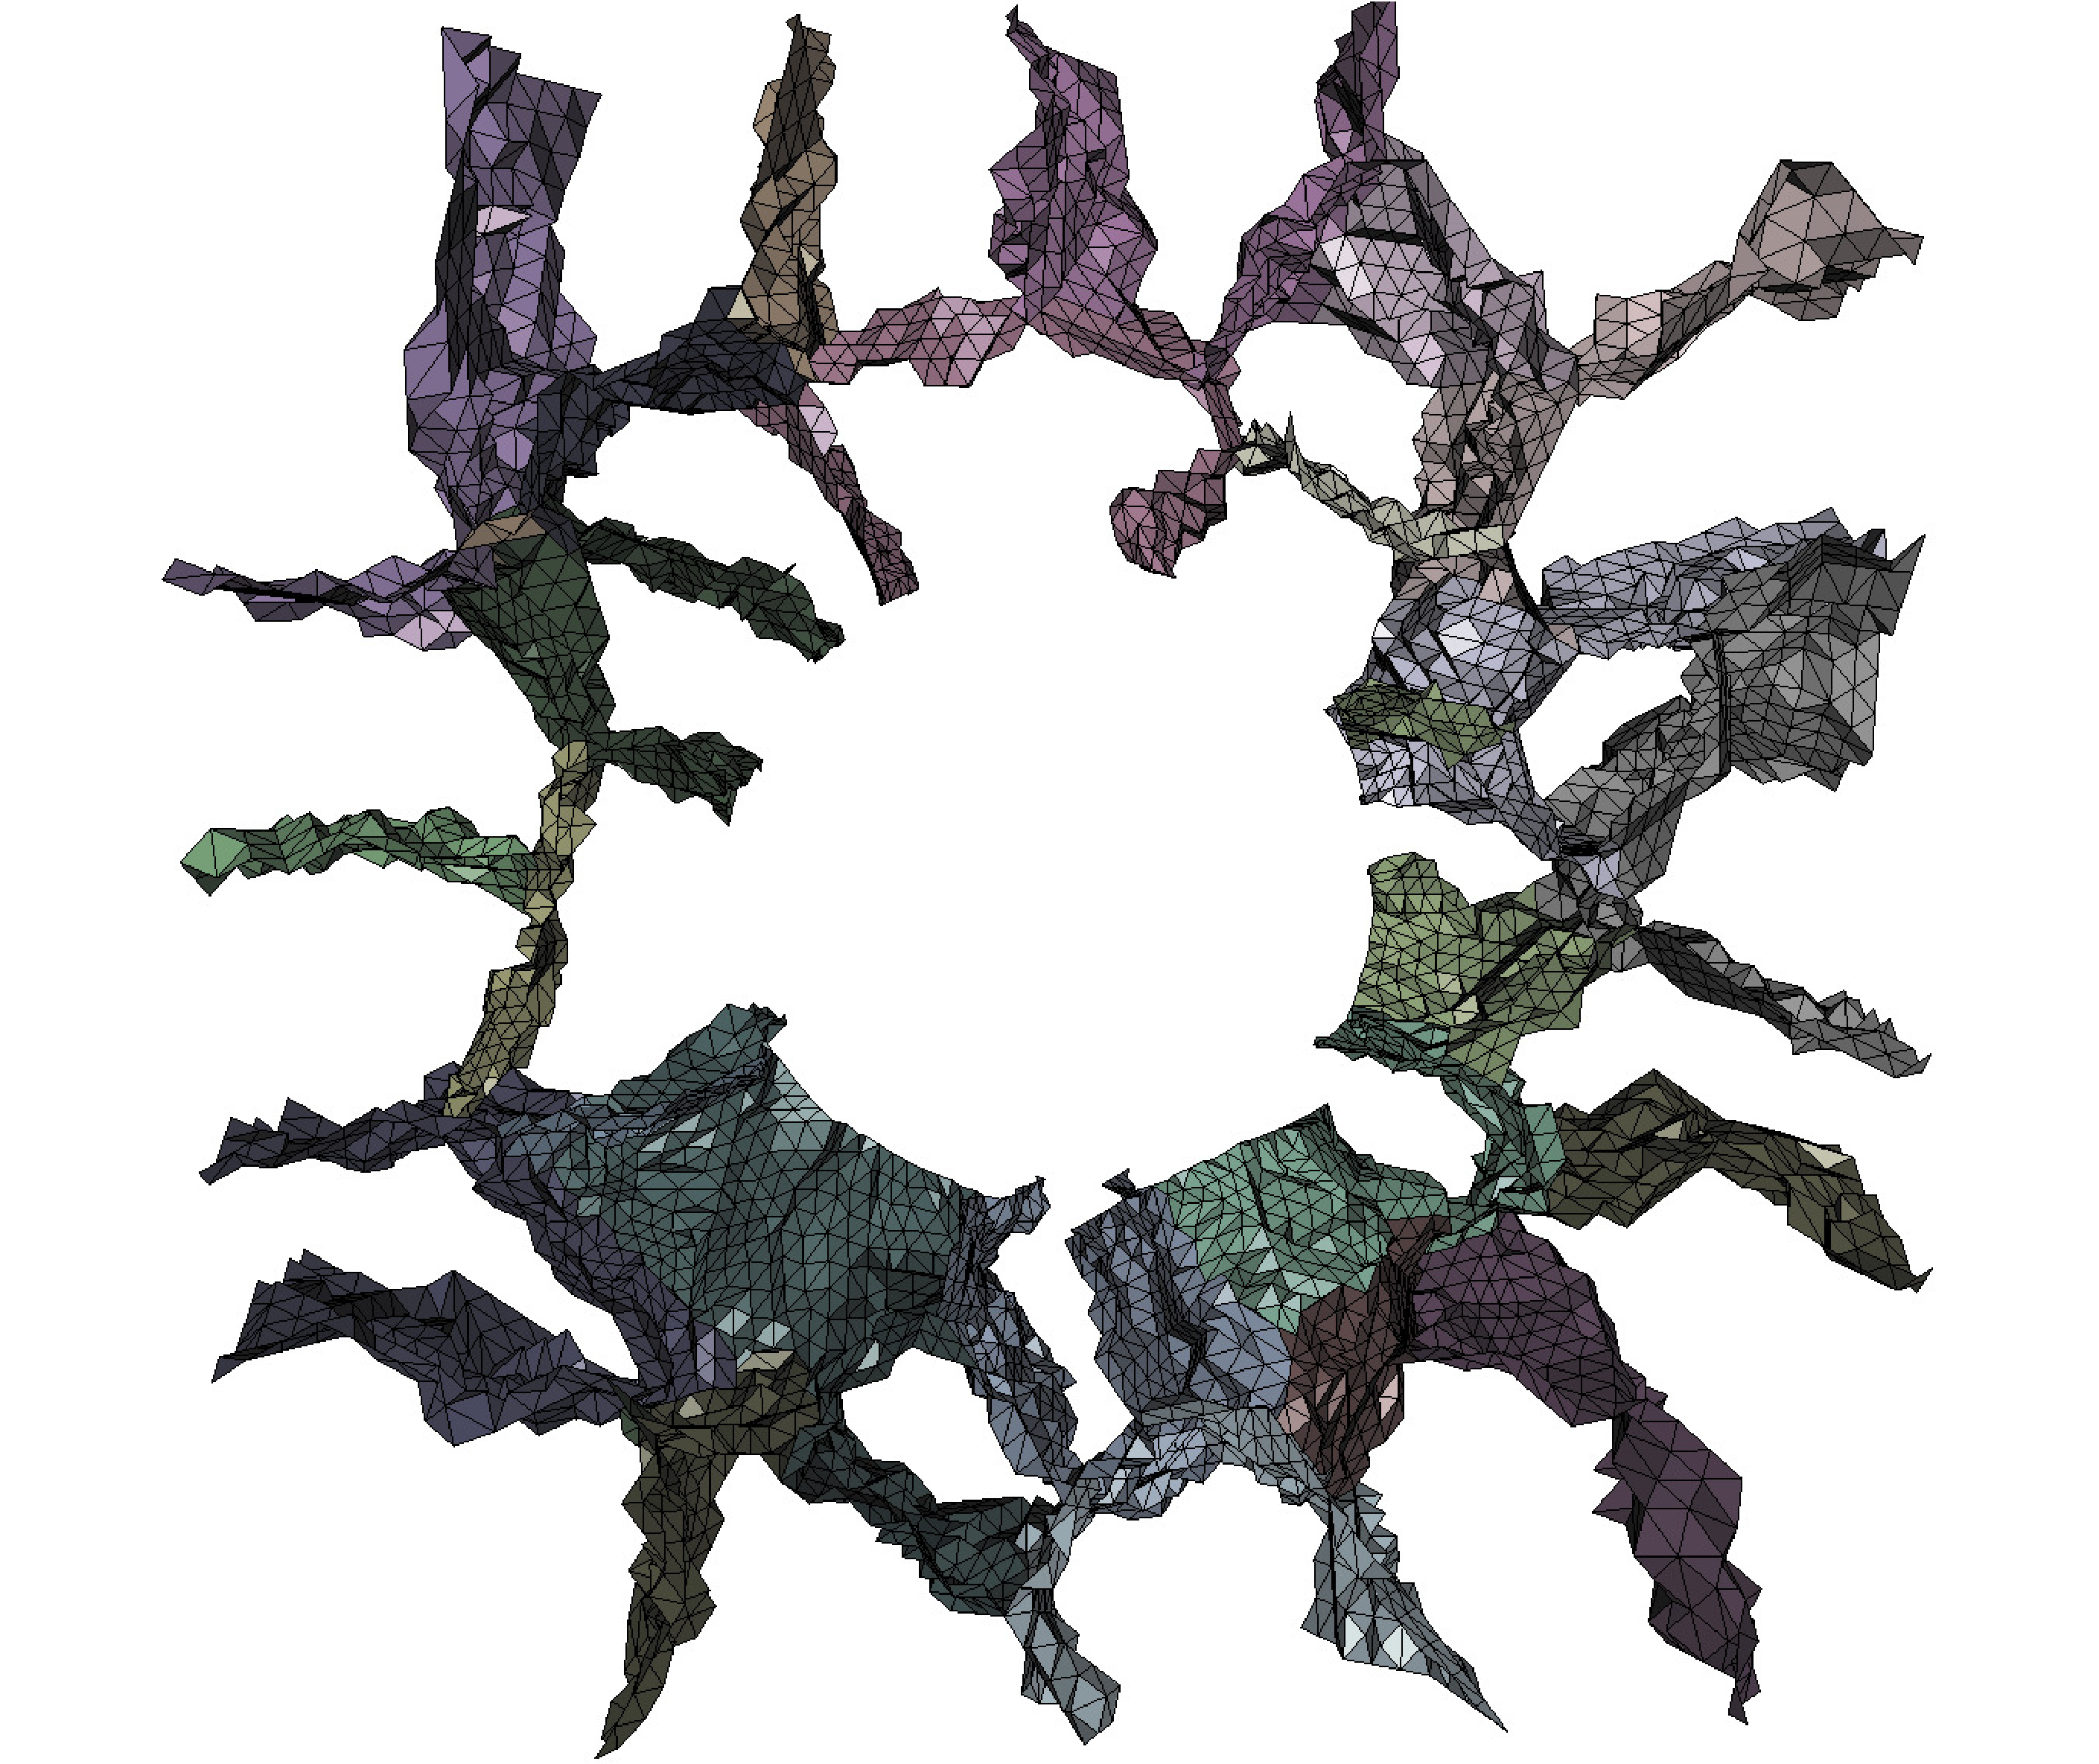
\includegraphics[width=2.3cm]{images/eps/rechteckring58534p_copy_entsaettigt3003.pdf}};


		\draw [arrow] (one) -- node[anchor=south] {\bf Decompose} (two);
		\draw [arrow, align=center, text width=2.3cm] (two) -- node[anchor=south] {\bf Build \mbox{alternative} problem} (three);
		\draw [arrow] (three) -- node[anchor=south] {\bf Linearize} (four);
	\end{tikzpicture}
\end{frame}

\begin{frame}{One-level nonlinear Schwarz \footnote{\tiny Cai and Keyes 2002}}%: Nonlinearly preconditioned inexact Newton algorithms}}
	% \only<1-3>{
		Discretized nonlinear partial differential equation: F (u) = 0
	    \vspace*{-5mm}
	% }
	% \only<4->{
	%     \vspace*{-10mm}
	% }

	\begin{columns}
		\begin{column}{0.5\textwidth}
			\begin{block}<1->{\normalsize Nonlinear corrections $T_i(u): V\mapsto V_i$}
				\vspace*{-5mm}
				\begin{align*}
					 & R_iF(u-P_iT_i(u))  = 0, \quad i = 1,2,\dots N                \\
					 & \text{with}\quad R_i:V\mapsto V_i\text{,}\, P_i:V_i\mapsto V
				\end{align*}
			\end{block}
		\end{column}
		\begin{column}{0.5\textwidth}
			\begin{block}<2->{\normalsize Define an alternative nonlinear problem}
				\begin{equation*}
					\mathcal{F}_1(u) \coloneqq \sum_{i=1}^N\alert<4>{P_iT_i(u)} = 0
				\end{equation*}
			\end{block}
		\end{column}
	\end{columns}
	\begin{block}<3->{\normalsize Nonlinear Schwarz method results by solving $\mathcal{F}_1(u) = 0$ with Newton's method.\newline Setting $u_i = u-P_iT_i(u)$ the Jacobian can be formulated as:}
		\vspace*{-2mm}
		\begin{align*}
			D\mathcal{F}_1(u^k)  = \sum_{i = 1}^NP_iDT_i(u^k) = \sum_{i=1}^N\alert<4>{P_i(R_iDF(u_i^k)P_i)^{-1}R_iDF(u_i^k)}
		\end{align*}
	\end{block}
	\only<4>{%
		\tikz[overlay,remember picture]
		\node[fill=white,text=red] at ([xshift=0cm,yshift=-3cm]current page.center){\Large Parallel execution!};
	}
	% \only<4>{%
	% \begin{itemize}
	% 	\item For the one-level nonlinear Schwarz method the solutions of $F(u) = 0$ and $\mathcal{F}_1(u) = 0$ are equivalent
	% 	\item The global operators $DF(u_i)$ only need to be assembled locally
	% \end{itemize}
	% }
\end{frame}


\begin{frame}{Two-level additive nonlinear Schwarz \footnote{\tiny Heinlein, Lanser (2020)} \footnote{\tiny Heinlein, Lanser, Klawonn (2022)}}
	% \vspace*{-5mm}
	\begin{columns}
		\begin{column}{0.5\textwidth}
			\begin{block}{\normalsize Nonlinear corrections $T_i(u)$}
				\vspace*{-1mm}
				\begin{align*}
					 & R_iF(u-P_iT_i(u))  = 0, \quad i = \alert{0},1,2,\dots N      \\
					 & \text{with}\quad R_i:V\mapsto V_i\text{,}\, P_i:V_i\mapsto V
				\end{align*}
			\end{block}
		\end{column}
		\begin{column}{0.5\textwidth}
			\begin{block}{\normalsize Alternative nonlinear problem}
				\begin{equation*}
					\mathcal{F}_A(u) \coloneqq \alert{P_0T_0(u)} + \sum_{i=1}^NP_iT_i(u) = 0
				\end{equation*}
			\end{block}
		\end{column}
	\end{columns}
	\begin{block}{\normalsize The Jacobian}
		\vspace*{-2mm}
		\begin{align*}
			D\mathcal{F}_A(u^k)  = \alert{P_0(R_0DF(u_0^k)P_0)^{-1}R_0DF(u_0^k)} + \sum_{i=1}^NP_i(R_iDF(u_i^k)P_i)^{-1}R_iDF(u_i^k)
		\end{align*}
	\end{block}
\end{frame}

\begin{frame}{Two-level hybrid nonlinear Schwarz  \footnote[2]{\tiny Heinlein, Lanser (2020)} \footnote[3]{\tiny Heinlein, Lanser, Klawonn (2022)}}
	\vspace*{-5mm}
	\begin{block}{\normalsize Alternative nonlinear problem}
		\begin{equation*}
			\mathcal{F}_{hybrid}(u) \coloneqq \sum_{i=1}^NP_iT_i(u-P_0T_0(u)) + P_0T_0(u),
		\end{equation*}
	\end{block}
	\begin{block}{\normalsize The Jacobian}
		\vspace*{-2mm}
		\begin{equation*}
			D\mathcal{F}_{hybrid}(u^k) = I - \left(I-\sum_{i=1}^NQ_i(v_i)\right)(I-Q_0(u_0))
		\end{equation*}
		\begin{align*}
			\text{with}\quad Q_i(u) & \coloneqq P_i(R_iDF(u)P_i)^{-1}R_iDF(u), \\
			u_i                     & \coloneqq u-P_iT_i(u)                    \\
			\text{and}\quad v_i     & \coloneqq u_0-P_iT_i(u_0)
		\end{align*}
	\end{block}
\end{frame}
